\documentclass[a4paper]{article}
\usepackage[T1]{fontenc}
\usepackage[utf8]{inputenc}
\usepackage[top=2cm, bottom=2cm, left=2cm, right=2cm]{geometry}
\usepackage{color}
\usepackage{url}
\usepackage{array}
\usepackage{pifont}
\usepackage{graphicx}
\setlength{\skip\footins}{2cm}

\title{COMP-512 Distributed Systems, Fall 2011}
\author{
Matthieu \textsc{Dubet} \\
Alexander \textsc{Kawrykow} \\ \\ \\
\emph{School of Computer Science, McGill University }
}

\begin{document}
\maketitle
\begin{figure}
  \centering
	
\includegraphics[scale=0.8]{mcgill_logo.png}
  \label{mcgill}
\end{figure}
\clearpage
\tableofcontents
\clearpage
%\section{Introduction}
\section{Project Part 1: Distributing an Application}
\subsection{Design}

We decided to separate the ResourceManager interface to split the concerns. 

Accordingly, we created one type of Interface for each kind of resource (room, car, flight, customer), and finally aggregated all these into one large interface (the IResourceManager). 

We then looked at the functionality common to anything Resource-Manager related: reading data, writing data, querying data, etc. In particular,
these are functions which have no semantic meaning specific to any of the resources. We extracted these into an AbstractResourceManager.
For each kind of resource, we implemented a concrete ResourceManager who was able to reuse the functionality in the AbstractResourceManager, 
but in the context of a particular resource. 


Both our RMI and TCP implementations of the ResourceManagers act as wrappers for their underlying ResourceManager. That is, a RMI car resource manager
takes care of binding to the registry and remote method calls, but the underlying logic happens by delegating to a concrete car resource manager. A
similiar approach was taken for the TCP car resource manager. In this way, we were able to maximize code reuse. 


Another step taken to maximize code reuse was our treatment of the Client. Rather than re-writing the client for TCP, we created a TCP "proxy" resource
manager which implements IResourceManager, but simply passes on the exact command to the remote middleware server. Here, the proxy is simply a local
reference we can create when the client is launched.


The remote middleware server listens for the TCP/IP messages, looks at the first few letters, and then delegates the exact command. For example, we know a command containing the substring "car" must be sent, via TCP/IP, to the car resource manager server, so little processing of the commands ever needs to take place. 

The car resource manager can then just look at the first few letters of his received command,
and delegate to his reference to a local concret car resourcemanager depending on the type of query. For example, if the command starts with 'new', we know
we can call the newCar method on the local reference and have him take care of the logic. 



To handle customers, we decided to treat the MiddleWare as a kind of resource manager himself. 

In both implementations, the Middleware server has a local reference to a CustomerResourceManager object to handle all of the logic pertaining to customers, as well as reservations and the itinerary feature. In the case of RMI, the CustomerResourceManager can use his remote object references to easily handle reservations. By contrast, for the TCP implementation, we had to reconstruct the objects the CustomerResourceManager would put in his hashtable. 

We did this by exchanging the objects over sockets in string form, as a list of attributes corresponding to the id, location, price, etc. For example, to reserve a car, the flow goes something like: send message to middleware, middleware constructs Car object by sending message to car resource manager to obtain the state of the specific car, middleware passes the car object to his local customer resource manager who places it in his hashtable to keep track of the reference. 


For the UML diagram, please refere to Figure~\ref{uml}.

\begin{figure}
  \centering
	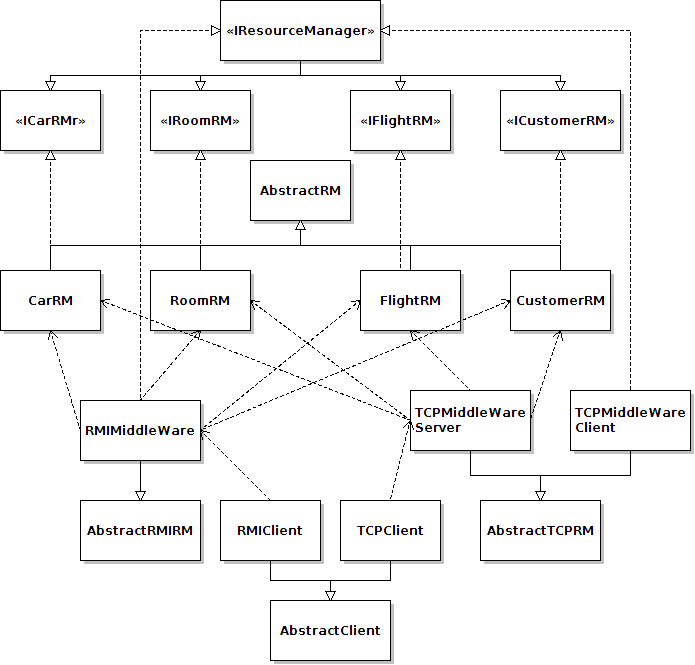
\includegraphics[scale=0.6,angle=90]{classhierarchy.png}
  \caption{UML Class Diagram}
  \label{uml}
\end{figure}


\subsection{Testing}
\subsubsection{Bash scripts}
To facilitate the testing of the system, Bash scripts are available.
\begin{itemize}
\item{
{\tt launch.sh [tcp/rmi] [car/room/flight/middleware] [port] [.....]}.

It take several arguments to launch each of the service (CarResourceManager,Room,Flight,Middleware or Client), either via TCP or RMI.
}
\item{
{\tt launch-localhost.sh [tcp/rmi] [portcar] [portroom] [portflight] [portmiddleware]}.

It deploys all the services all at a time on localhost.
}
\item{
{\tt launch-client.sh [tcp/rmi] [host:port]} is used to launch a client (either RMI or TCP) 
allowing fast testing when it's combined with the {\tt input1} file which contains multiple testcases.
}
\end{itemize}

\subsubsection{Example}
A traditional runcase with 3 servers would be :

First, login to server1 and launch all the resource managers.

{\tt ./launch.sh rmi flight 2000}

{\tt ./launch.sh rmi car 2001}

{\tt ./launch.sh rmi room 2002}

Then, login to server2 and launch the middleware.

{\tt ./launch.sh rmi middleware 2003 -flight=server1:2000 -car=server1:2001 -room=server1:2002}

Finaly, login to server3 and use the client redirecting stdin from the input1 file
 
{\tt ./launch-client.sh rmi server2:2003 < input1}

\section{Project Part 2: Transactions and Concurrency Control}
\subsection{Design}
\subsubsection{General}

Recall that for each resource manager, a hierarchy such shown in figure \ref{carrm} exists. To maximize code reusibility, both the \texttt{RMICarRM} and \texttt{TCPCarRM} pose as resource managers but delegate to a local instance of 
\texttt{CarRM} which implements concrete logic describing how cars should be managed. 
\begin{figure}[h!]
  \centering
	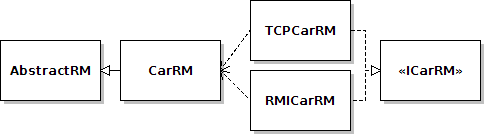
\includegraphics[scale=0.6]{carrm.png}
  \caption{ResourceManager hierarchy}
  \label{carrm}
\end{figure}
We noticed that we could support transaction support for \it both \rm TCP and RMI, \bf for free\rm, if transaction management was implemented at the \texttt{CarRM} level. Accordingly, we defined a new interface \texttt{ITransactionManager} which 
exposes the set of methods prescribed in the assignment and had both \texttt{RMICarRM} and \texttt{TCPCarRM} implement this interface. Again, we maximized code reuse by delegating to the concrete \texttt{CarRM} for handling transactions
rather than redoing it for both TCP and RMI. Likewise, we noticed that the set of methods exposed by the \texttt{ITransactionManager} was exactly the same for all of the resource managers. That is, a \texttt{commit} always:
\begin{enumerate}
 \item[1.] Removes the transaction from the list of active transactions 
 \item[2.] Unlocks all resources held by that transaction
\end{enumerate}
Similarly, an \texttt{enlist} adds the transaction to the list of active transactions, while an \texttt{abort} always: does a rollback, remove from active transaction list, unlock resources. The datatstructures involved are the same
regardless of resource manager type. Consequently, these methods were all implemented \texttt{AbstractRM} and inherited by the concrete RMs. Adding transaction support, then, simply involved adding a few lines to each method of each RM:
\begin{enumerate}
 \item[1.] Check if the given \texttt{TxID} is in the list of active transactions, and throw an \texttt{InvalidTransactionException} if not
 \item[2.] For a write, load the appropriate UNDO op (see section \ref{rollbacks})
 \item[3.] Lock the resource, uniquely identified by the Key (for example, this key is the \texttt{location} parameter for the car RM).
\end{enumerate}
In this way, the middleware only needed to be modified slightly: upon receiving, for example, a query for a car's price, we call the remote car RM's method and only need to worry about catching the appropriate exceptions. For example, if a 
\texttt{DeadLockException} is thrown, we tell all RM's to abort. In this way, each resource manager worries only about locking their own kind of resource, rather than a centralized transaction manager worrying about all the resources.
Likewise, each resource manager has its own \texttt{LockManager} instance for locking, rather than a centralized lock manager. A glimpse of the updated design is provided in figure \ref{txncarrm}
\begin{figure}[h!]
  \centering
	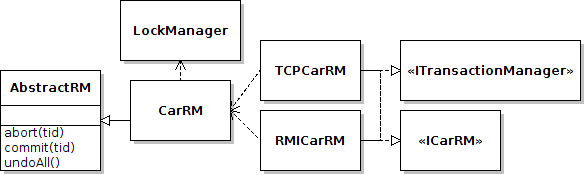
\includegraphics[scale=0.6]{txncarrm.png}
  \caption{Updated ResourceManager hierarchy}
  \label{txncarrm}
\end{figure}
\subsubsection{Rollbacks}
\label{rollbacks}

A rollback consists of sequential execution of inverse operations. For example, the inverse of an \texttt{ADD} is a \texttt{DELETE} (and vice-versa), and the inverse of a \texttt{WRITE} is a \texttt{WRITE} containing the old values. 
We defined a generic \texttt{Operation} class which encapsulates this concept. Each instance of \texttt{Operation} contains a type (one of \texttt{ADD}, \texttt{DELETE}, \texttt{WRITE}, \texttt{UNRESERVE}) as well as a key-value pair
which describes the operation. For example, an \texttt{ADD} consists of the key of the object (location in the case of cars), and a value consisting of the object to write itself. 

Each RM maintains, for each active transaction, a \texttt{Stack<Operation>} onto which he pushes inverse operations prior to any writes. The \texttt{AbstractRM}'s \texttt{undoAll(txID)} method then keeps popping off the appropriate stack
and `performing' the inverse operations until none are left. 

\subsection{Performance evaluation}
The goals of having a distributed system instead of a more traditional monolithic one is mainly to achieve fault-tolerance and scalability.

In this section, we will submit our system to different kinds of benchmarks to see how scalable it is.

From a client point of view, we measure the time between the start and the commit(or the abort) of a transaction on different tests bench.
On each bench, we try several transaction types :
\begin{itemize}
\item Small transaction not distributed (3 operations on the same RM)
\item Small transaction distributed (3 operations on 3 different RMs)
\item Big transaction not distributed (9 operations on the same RM)
\item Big transaction distributed (9 operations on 3 different RMs)
\end{itemize}

In the first benchmark, we try only one client (no concurrency) and one server hosting all RMs with various throughput.
\begin{figure}[h!]
  \centering
	\includegraphics[scale=0.6]{one_client.png}
  \caption{One client performance evaluation (response time in microseconds function of throughput)}
  \label{oneclient}
\end{figure}

As we see, the response time for each transaction types are pretty much constant, whatever the throughput is. It is easily explained by the fact that  
%\bibliographystyle{plain}
%\bibliography{bib}
\end{document}
